\documentclass[conference]{IEEEtran} % Usa la classe IEEEtran per formattazione simile

\usepackage{amsmath}
\usepackage{graphicx}



\begin{document}

\title{Exploring the Adversarial Robustness of AI-generated Image Detectors}

\author{
    \IEEEauthorblockN{Thomas Lazzerini, Samuele Cappelletti, Martina D'Angelo}
    \IEEEauthorblockA{
        University of Trento
    }
}

\maketitle

\begin{abstract}
Semi-supervised image classification is a machine-learning task in which a model is trained using a combination of labeled and unlabeled data. This paper consists of a high-level survey of semi-supervised image classification literature and expands on its main theoretical and practical challenges, providing a taxonomy of the most popular semi-supervised learning algorithms. ciao come va
\end{abstract}

\section{Introduction}
Semi-supervised image classification is nowadays a hot research topic. The objective is to tackle the major issue of Supervised Learning: the scarcity of labeled data...
% Continua con il tuo contenuto

As discussed in \cite{zhu2005semi}, semi-supervised learning is an important area of research.

\begin{figure}[h]
    \centering
    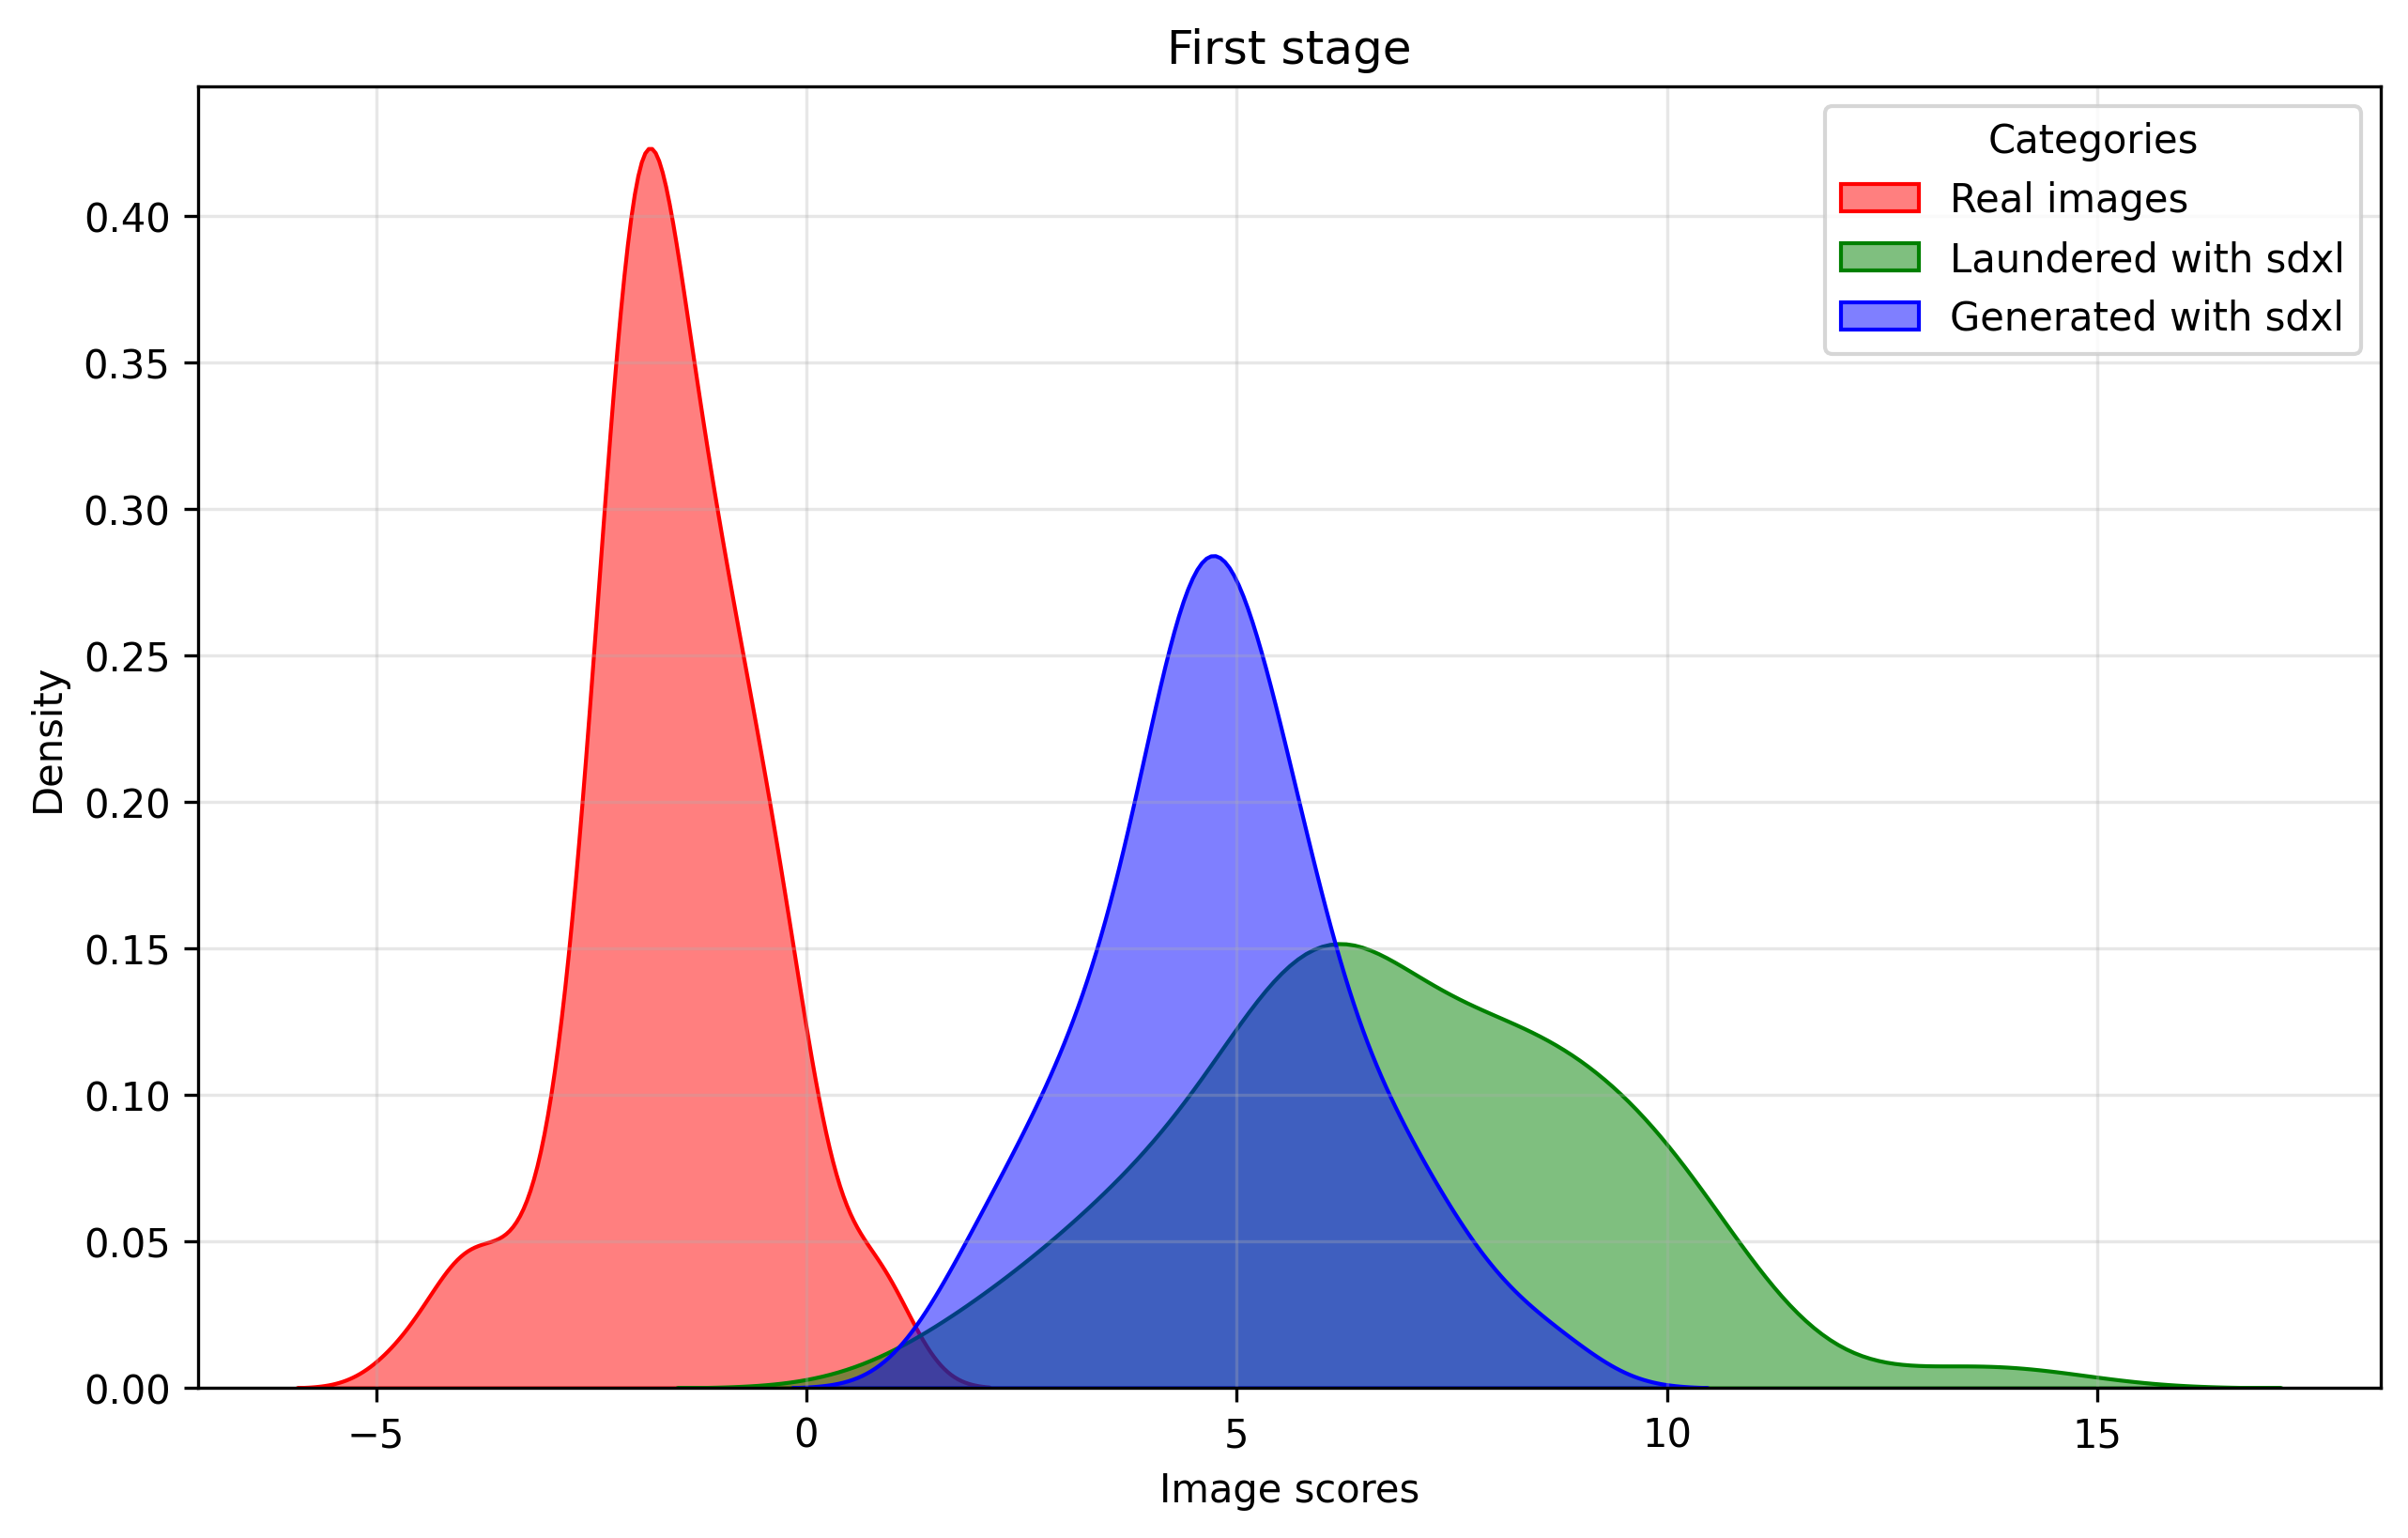
\includegraphics[width=0.8\linewidth]{Img/First_stage.png}
    \caption{Esempio di immagine.}
    \label{fig:esempio}
\end{figure}


\section{Detectors}
    \subsection{CLIP}
    \subsection{PIZZA}
\section{Attacks}
    \subsection{Mimicry}
    \subsection{SD Laundering}
    \subsection{White Black}
    \subsection{Adversarial Robustness}
\section{Experiment}
\section{Conclusions}

\bibliographystyle{IEEEtran} % Stile delle referenze (es. IEEE)
\bibliography{references}    % Nome del file .bib (senza estensione)

\end{document}